\documentclass{beamer}

% Main theme configuration
\usetheme{ucl}
\useoutertheme[small]{ucltitlebanner}
\setbeamercolor{banner}{bg=darkblue}

% Packages and settings
\graphicspath{{./fig_final_report/}{./fig_paper/}{./fig/}}

% Set a smaller indent for description environment
\setbeamersize{description width=2em}

% Remove nav symbols (and shift any logo down to corner)
\setbeamertemplate{navigation symbols}{\vspace{-2ex}}

% Title slide logos
\newlength{\titlegraphicheight}
\setlength{\titlegraphicheight}{0.15\paperheight}
\titlegraphic{%
	\includegraphics[height=\titlegraphicheight]{cdt_dis_logo}%
	\hspace{15pt}%
	\includegraphics[height=\titlegraphicheight]{ukaea_logo}%
}

% Metadata
\title[Surrogate Modelling of the Tritium Breeding Ratio]{Surrogate Modelling of the Tritium Breeding Ratio}
\author[Petr Mánek \and Graham Van Goffrier]{Petr Mánek \and Graham Van Goffrier}
\institute[UCL]{%
	Centre for Doctoral Training in Data Intensive Science \\ %
	University College London
}
\date{22nd June 2020}

\begin{document}

% Title slide
\begin{frame}
  \titlepage%
\end{frame}

% Body of the presentation is organized in separate files
\section{Introduction}
%TODO: make all more concise, bullet points

\begin{frame}
	\frametitle{Project Background}
	Nuclear fusion -- the energy of the future!
    \vspace{10pt}
	\begin{itemize}
	    \item Must produce and contain an extremely hot and dense plasma
	    \begin{itemize}
		    \item Magnetic Confinement Fusion (MCF): toroidal circulation
		    \item Inertial Confinement Fusion (ICF): spherical compression
		\end{itemize}
		\vspace{10pt}
		\item Modern designs require enriched Hydrogen fuel of two varieties:
	    \begin{itemize}
		    \item Deuterium ($^2$H) -- abundant in naturally-sourced water.
		    \item Tritium ($^3$H) -- extremely rare, but can be produced \textit{in-reactor}.
		\end{itemize}
	\end{itemize}
	\vspace{10pt}
	\centering{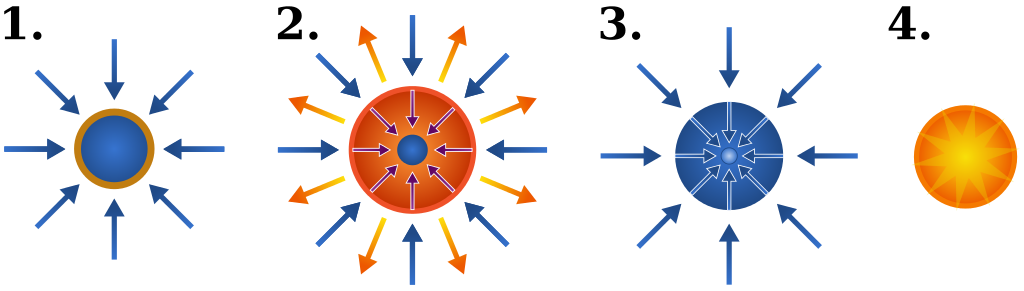
\includegraphics[height=3cm]{icf_diagram}}
\end{frame}

\begin{frame}
	\frametitle{Problem Description}
	Tritium breeding blankets convert neutron radiation to tritium fuel:
	\begin{align*}
		\isotope[1][0]{n} + \isotope[6][3]{Li} \rightarrow \isotope[3][1]{H} +
		\isotope[4][2]{He}
		\qquad\qquad
		\isotope[1][0]{n} + \isotope[7][3]{Li} \rightarrow \isotope[3][1]{H} +
		\isotope[4][2]{He} + \isotope[1][0]{n}
	\end{align*}
	Tritium breeding ratio (TBR) = fuel bred / fuel consumed
	
	\begin{itemize}
	    \item Depends on numerous geometric and material parameters.
	    \item Evaluated precisely by OpenMC neutronics simulation \textit{Paramak}, but is computationally expensive. 
	\end{itemize}
	
	\vspace{15pt}
	
	\begin{block}{Our Challenge:}
		\begin{center}
			Produce a fast TBR function that strongly approximates Paramak, making use of the latest in surrogate modelling techniques.
		\end{center}
	\end{block}
\end{frame}

\begin{frame}
	\frametitle{Data Generation}
	We produced training and test datasets by uniform random sampling over the 7
	discrete and 11 continuous parameters of Paramak.

	\begin{columns}[T]
		\column{0.34\textwidth}

		\vspace{5pt}

		Paramak was deployed on UCL's Hypatia cluster:
		\begin{itemize}
		\item Generated 1M samples.
		\item 27 days of runtime.
		\end{itemize}

		\vspace{5pt}

		2~classes of runs:
		\begin{itemize}
		\item All parameters free.
		\item Discrete fixed, continuous free.
		\end{itemize}

		\vspace{5pt}

		{\footnotesize
		Groups of fractions marked\textsuperscript{\textdagger\textdaggerdbl} are required to sum to 1.
		}

		\column{0.62\textwidth}
		\vspace{5pt}

		{\fontsize{8pt}{8pt}\selectfont
		\setlength\tabcolsep{3pt}
		\begin{tabular}{l|ll}
		\toprule
		{} & Parameter name & Domain\\
		\midrule
		\parbox[t]{2mm}{\hspace{-2pt}\multirow{12}{*}{\rotatebox[origin=c]{90}{Blanket}}}
		   & Breeder fraction\textsuperscript{\textdagger} & $[0,1]$\\
		   & Breeder \isotope[6]{Li} enrichment fraction & $[0,1]$\\
		   & Breeder material & $\{\text{Li}_2\text{TiO}_3, \text{Li}_4\text{SiO}_4\}$\\
		   & Breeder packing fraction & $[0,1]$\\
		   & Coolant fraction\textsuperscript{\textdagger} & $[0,1]$\\
		   & Coolant material & $\{\text{D}_2\text{O}, \text{H}_2\text{O}, \text{He}\}$\\
		   & Multiplier fraction\textsuperscript{\textdagger} & $[0,1]$\\
		   & Multiplier material & $\{\text{Be}, \text{Be}_{12}\text{Ti}\}$\\
		   & Multiplier packing fraction & $[0,1]$\\
		   & Structural fraction\textsuperscript{\textdagger} & $[0,1]$\\
		   & Structural material & $\{\text{SiC}, \text{eurofer}\}$\\
		   & Thickness & $[0,500]$\\
		\midrule
		\parbox[t]{2mm}{\hspace{-2pt}\multirow{6}{*}{\rotatebox[origin=c]{90}{First wall}}}
		   & Armour fraction\textsuperscript{\textdaggerdbl} & $[0,1]$\\
		   & Coolant fraction\textsuperscript{\textdaggerdbl} & $[0,1]$\\
		   & Coolant material & $\{\text{D}_2\text{O}, \text{H}_2\text{O}, \text{He}\}$\\
		   & Structural fraction\textsuperscript{\textdaggerdbl} & $[0,1]$\\
		   & Structural material & $\{\text{SiC}, \text{eurofer}\}$\\
		   & Thickness & $[0,20]$\\
		\bottomrule
		\end{tabular}
		}

    \end{columns}
\end{frame}

%\begin{frame}
%	\frametitle{Dimensionality Reduction}
%	\begin{itemize}
%		\item % TODO
%	\end{itemize}
%\end{frame}

\begin{frame}
	\frametitle{Methodology}
		Conventional regression task -- search for a cheap surrogate $\hat{f}(x)$ that
		minimizes dissimilarity with an expensive function $f(x)$:

		\begin{itemize}
			\item
				Regression performance: mean absolute error, $\sigma$ of
				error, $R^2$, $R^2_\text{adj.}$
			\item
				Computational complexity:
				training \& prediction time / sample
		\end{itemize}

		\vspace{2em}

		2 approaches for surrogate training:
		\begin{enumerate}
			\item
				Decoupled -- trains models from previously sampled
				datapoints.
			\item
				Adaptive -- repeats sampling \& model training, increases
				sampling density in low-performance regions.
		\end{enumerate}
\end{frame}



\section{Decoupled Approach}
\begin{frame}
	\frametitle{Outline}
	Compare 9~state-of-the-art surrogate families in 4~experiments:
	
	\begin{enumerate}
		\item
			Hyperparameter tuning (simplified) -- Bayesian optimization,
			discrete features fixed \& withheld.
		\item
			Hyperparameter tuning -- same as \#1 but with all features.
		\item
			Scaling benchmark -- increase training set size.
		\item
			Model comparison -- train surrogates for practical use.
	\end{enumerate}
\end{frame}

\begin{frame}
	\frametitle{Experiments 1 \& 2: Hyperparameter Tuning}

	\begin{minipage}{0.32\textwidth}
		\begin{center}
			\footnotesize
			\hspace{5pt} Experiment~1, slice~(a)
			\vspace{-10pt}
		\end{center}
		\includegraphics[height=95pt]{exp1_slice0}
	\end{minipage}
	\begin{minipage}{0.32\textwidth}
		\begin{center}
			\footnotesize
			\hspace{5pt} Experiment~1, slice~(b)
			\vspace{-10pt}
		\end{center}
		\includegraphics[height=95pt]{exp1_slice1}
	\end{minipage}
	\begin{minipage}{0.32\textwidth}
		\begin{center}
			\footnotesize
			\hspace{5pt} Experiment~1, slice~(c)
			\vspace{-10pt}
		\end{center}
		\includegraphics[height=95pt]{exp1_slice2}
	\end{minipage}

	\begin{columns}
		\column{0.28\textwidth}
		\includegraphics[height=95pt]{exp2_time_vs_reg}
		\begin{center}
			\footnotesize
			\vspace{-10pt}
			\hspace{20pt} Experiment~2
		\end{center}

		\column{0.72\textwidth}
		\begin{itemize}
			\item
				Plots show $\overline{t}_\text{pred.}$ vs.~$R^2$ for 20 best surrogates per family (fastest, most
				accurate = top left).
			\item
				Omitting discrete features yields only a negligible
				improvement in performance.
			\item
				Overall dominated by tree-based surrogates (GBTs, ERTs) and
				neural networks.
		\end{itemize}
	\end{columns}

\end{frame}

\begin{frame}
	\frametitle{Experiment 3: Scaling Benchmark}
	\begin{columns}
		\column{0.5\textwidth}
		\begin{itemize}
			\item
				We observe a hierarchy.
			\item
				Best-performing families from the previous experiments also scale the
				best in $\overline{t}_\text{pred.}$.
			\item
				More samples: neural networks outperform tree-based models.
		\end{itemize}

		\column{0.5\textwidth}
		\begin{itemize}
			\item
				Instance-based surrogates (KNN, IDW) train trivially but have
				complex lookup.
			\item
				Neural networks show inverse scaling due to
				parallelization.
		\end{itemize}
	\end{columns}

	\vspace{1em}

	\begin{minipage}{0.32\textwidth}
		\includegraphics[height=95pt]{scaling_metric_r2}
		\begin{center}
			\footnotesize
			\vspace{-10pt}
			\hspace{5pt} Regression performance
		\end{center}
	\end{minipage}
	\begin{minipage}{0.32\textwidth}
		\includegraphics[height=95pt]{scaling_time_train}
		\begin{center}
			\footnotesize
			\vspace{-10pt}
			\hspace{5pt} Training time / sample
		\end{center}
	\end{minipage}
	\begin{minipage}{0.32\textwidth}
		\includegraphics[height=95pt]{scaling_time_pred}
		\begin{center}
			\footnotesize
			\vspace{-10pt}
			\hspace{5pt} Prediction time / sample
		\end{center}
	\end{minipage}

\end{frame}

\begin{frame}
	\frametitle{Experiment 4: Model Comparison}
	\begin{columns}
		\column{0.7\textwidth}
		\begin{itemize}
			\item
				Trained 8~models for practical use.
			\item
				Plots show true vs.~predicted TBR by Models~1, 2 \& 4,
				coloured by density.
			\item
				Best regression performance:
				\begin{itemize}
					\item
						Model 1: ANN, 500K~samples.
					\item
						$R^2=\num{0.998}$,
						$\sigma=\num{0.013}$,
					\item
						$\overline{t}_{\text{pred.}}=\SI{1.124}{\micro\second}$,
						$\num{6916416} \times$~faster.
				\end{itemize}
			\item
				Fastest prediction:\textsuperscript{\textdagger}
				\begin{itemize}
					\item
						Model 2: ANN, 500K~samples.
					\item
						$R^2=\num{0.985}$,
						$\sigma=\num{0.033}$,
					\item
						$\overline{t}_{\text{pred.}}=\SI{0.898}{\micro\second}$,
						$\num{8659251} \times$~faster.
				\end{itemize}
			\item
				Smallest training set:\textsuperscript{\textdagger}
				\begin{itemize}
					\item
						Model 4: GBT, 10K~samples.
					\item
						$R^2=\num{0.913}$,
						$\sigma=\num{0.072}$,
					\item
						$\overline{t}_{\text{pred.}}=\SI{6.125}{\micro\second}$,
						$\num{1269777} \times$~faster.
				\end{itemize}
		\end{itemize}

		{\footnotesize
			\textsuperscript{\textdagger}
			with acceptable regression performance.
		}

		\column{0.3\textwidth}
		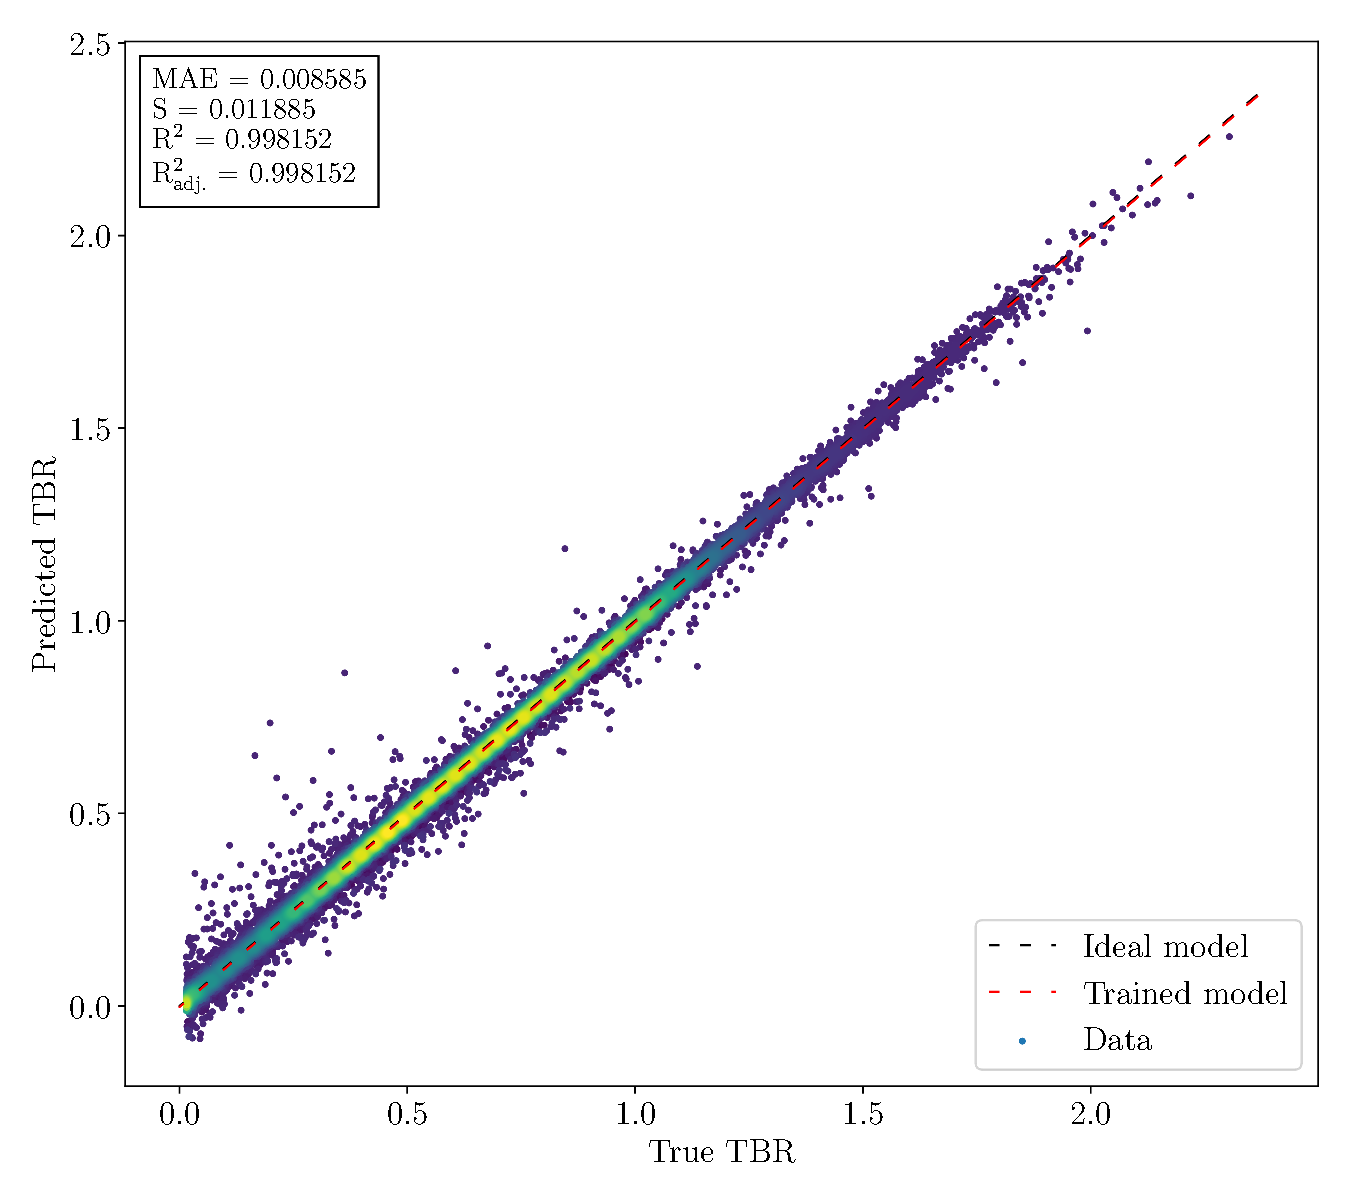
\includegraphics[height=83pt]{exp4_model6_rasterized}\vspace{-8pt}\\
		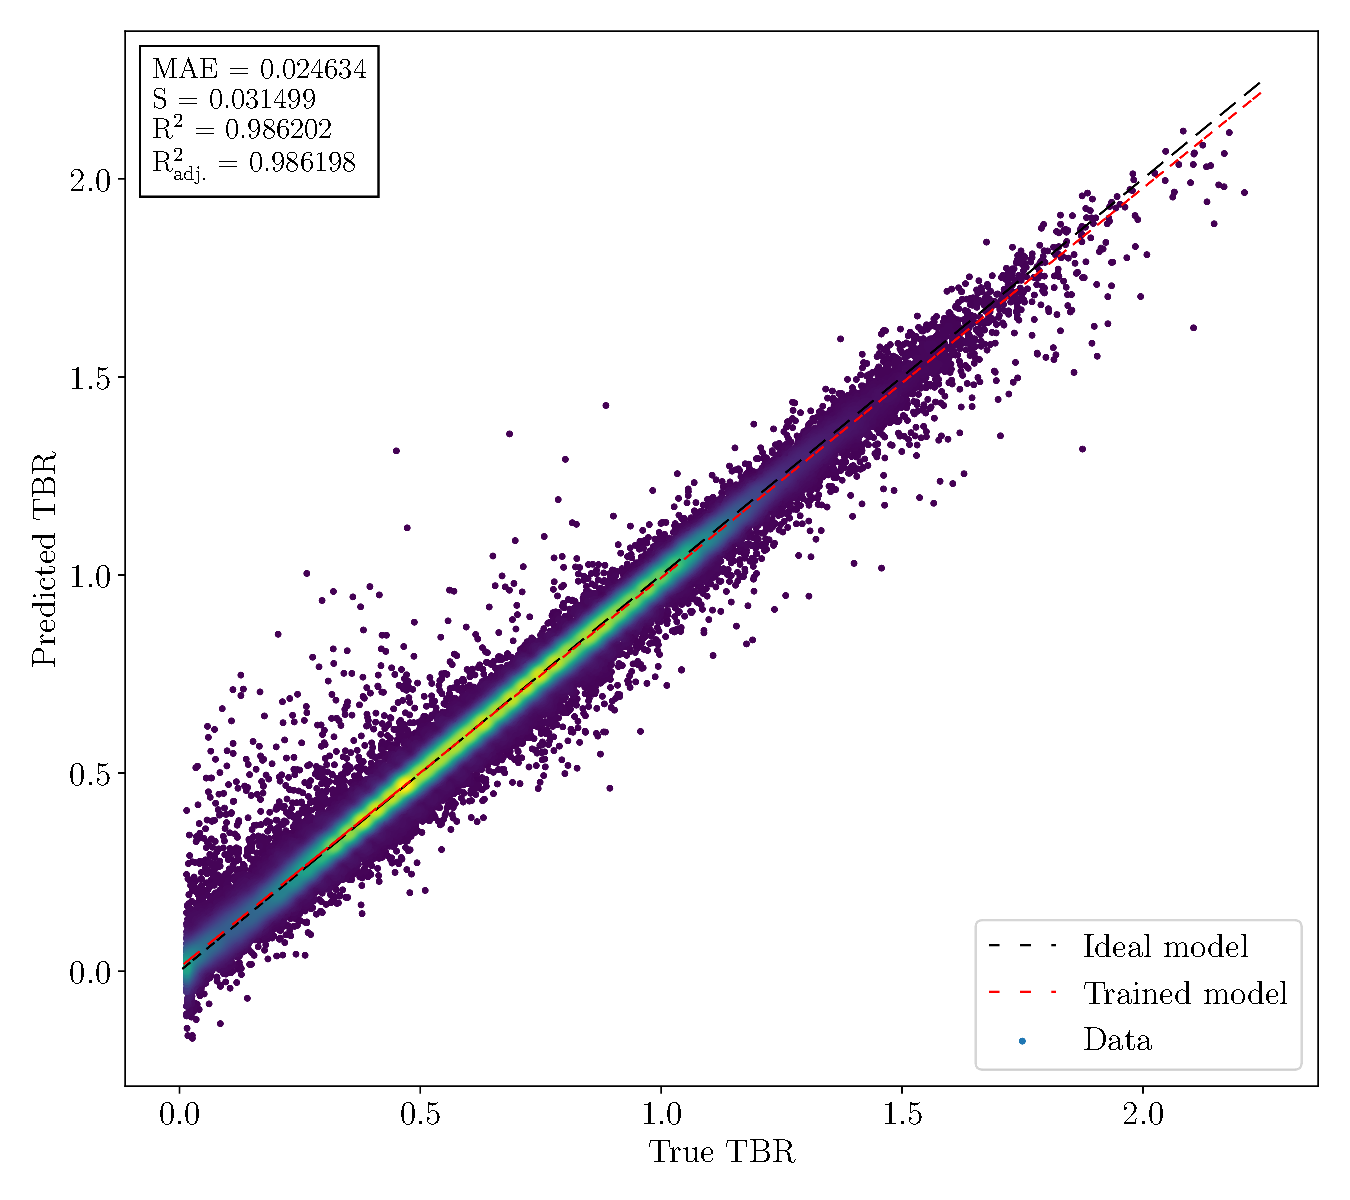
\includegraphics[height=83pt]{exp4_model7_rasterized}\vspace{-8pt}\\
		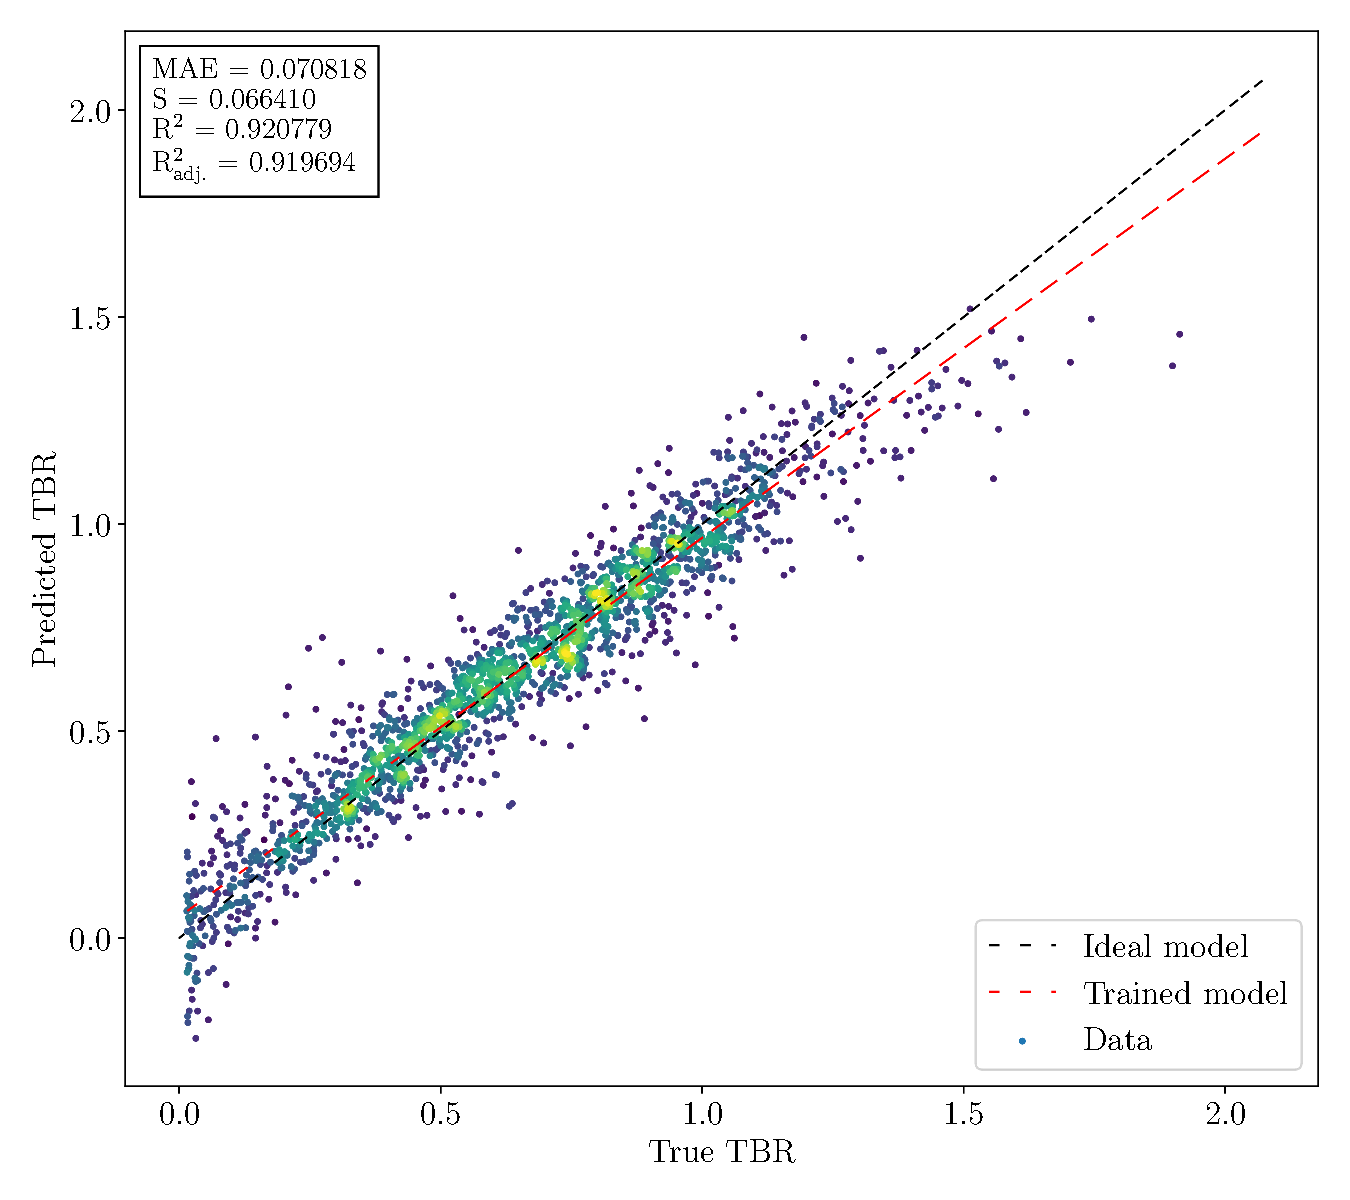
\includegraphics[height=83pt]{exp4_model3_rasterized}

		% TODO: remove some plots
		% TODO: say that we are showing only a subset
	\end{columns}
\end{frame}


\section{Adaptive Approach}
\begin{frame}
	\frametitle{Adaptive Sampling: Theory}
	 \begin{columns}[onlytextwidth,T]
      \column{\dimexpr\linewidth-6cm-5mm}
        
        Adaptive sampling takes advantage of surrogate information content \textit{during training} to reduce sample quantity.\newline
        
        We developed a new technique:
        \vspace{-5pt}
        \begin{enumerate}
        \item Construct surrogate quality distribution by nearest- neighbour interpolation.
        \item Draw candidate samples by quality using MCMC.
        \item Include samples with high crowding distance.
        \item Repeat!
        \end{enumerate}
      \column{6cm}
      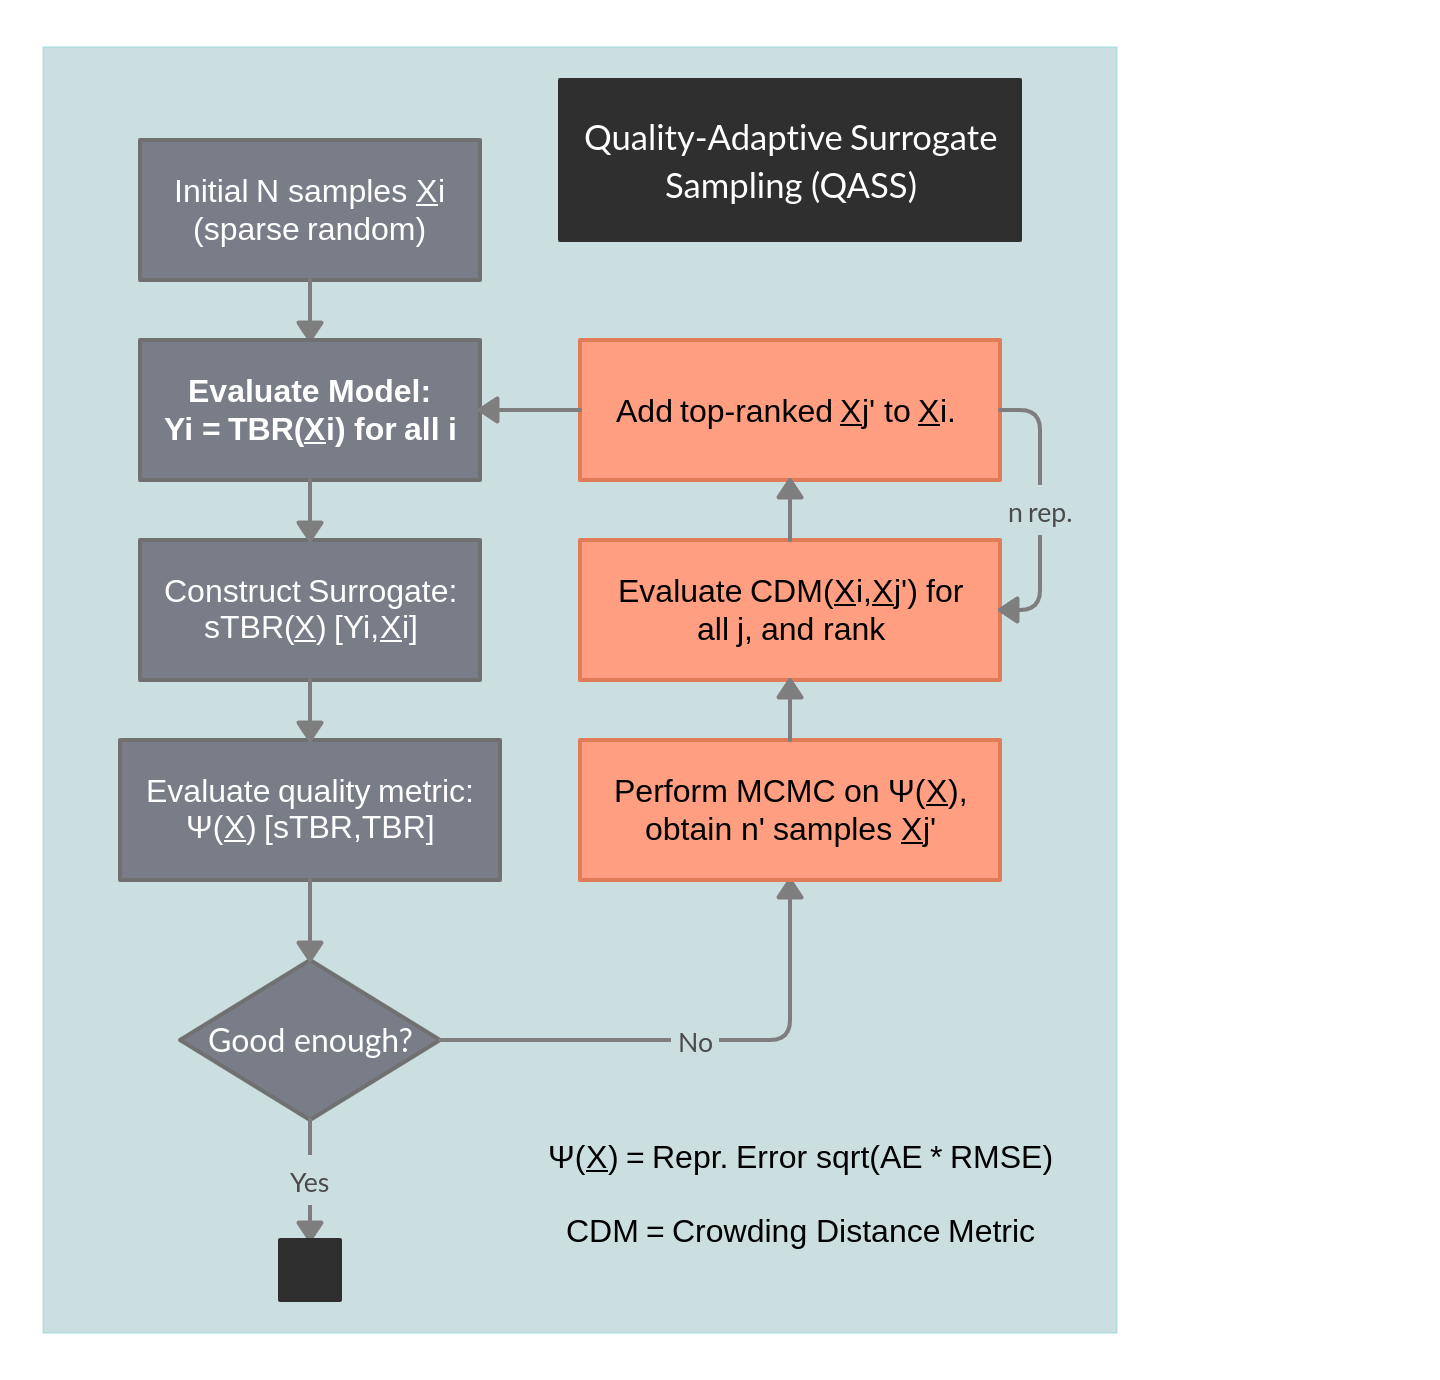
\includegraphics[width=8cm]{qassplan}

    \end{columns}
\end{frame}

\begin{frame}
	\frametitle{Application on Toy Theory}
	Toy functional TBR theory with wavenumber n, and similar ANN performance to Paramak:
	\begin{align*}
		\text{TBR} = \frac{1}{|C|}\sum_{i \in C} \left[1 + \sin(2\pi n (x_i - 1/2)) \right]
	\end{align*}

	\vspace{1em}

	\begin{columns}[T]
		\column{0.5\paperwidth}
		\vspace{0.5em}
		Two evaluation sets:
		\begin{itemize}
		    \item Adaptively-sampled dataset
		    \item Independent random dataset
		\end{itemize}
		\vspace{15pt}

		Placebo comparison -- a baseline scheme without MCMC, incremental uniform-random samples.


		\column{0.4\paperwidth}
		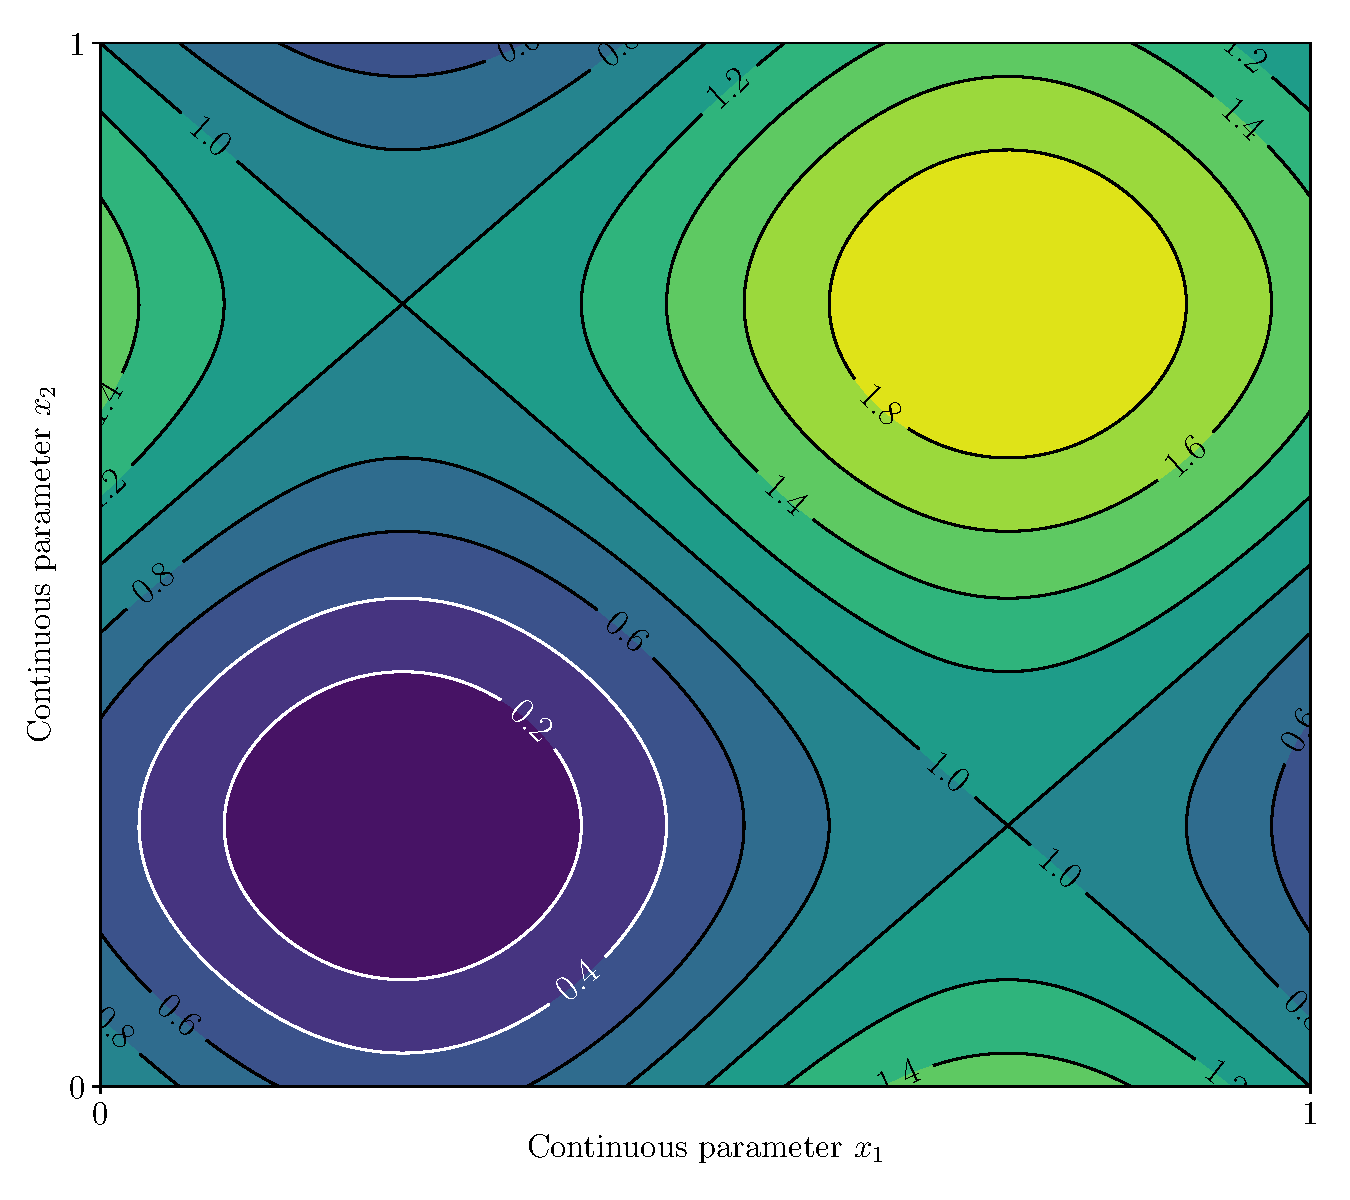
\includegraphics[width=0.4\paperwidth]{sintoy}

	\end{columns}
\end{frame}

\begin{frame}
    \frametitle{Adaptive Sampling: Results}
    \vspace{-10pt}
    \begin{center}
    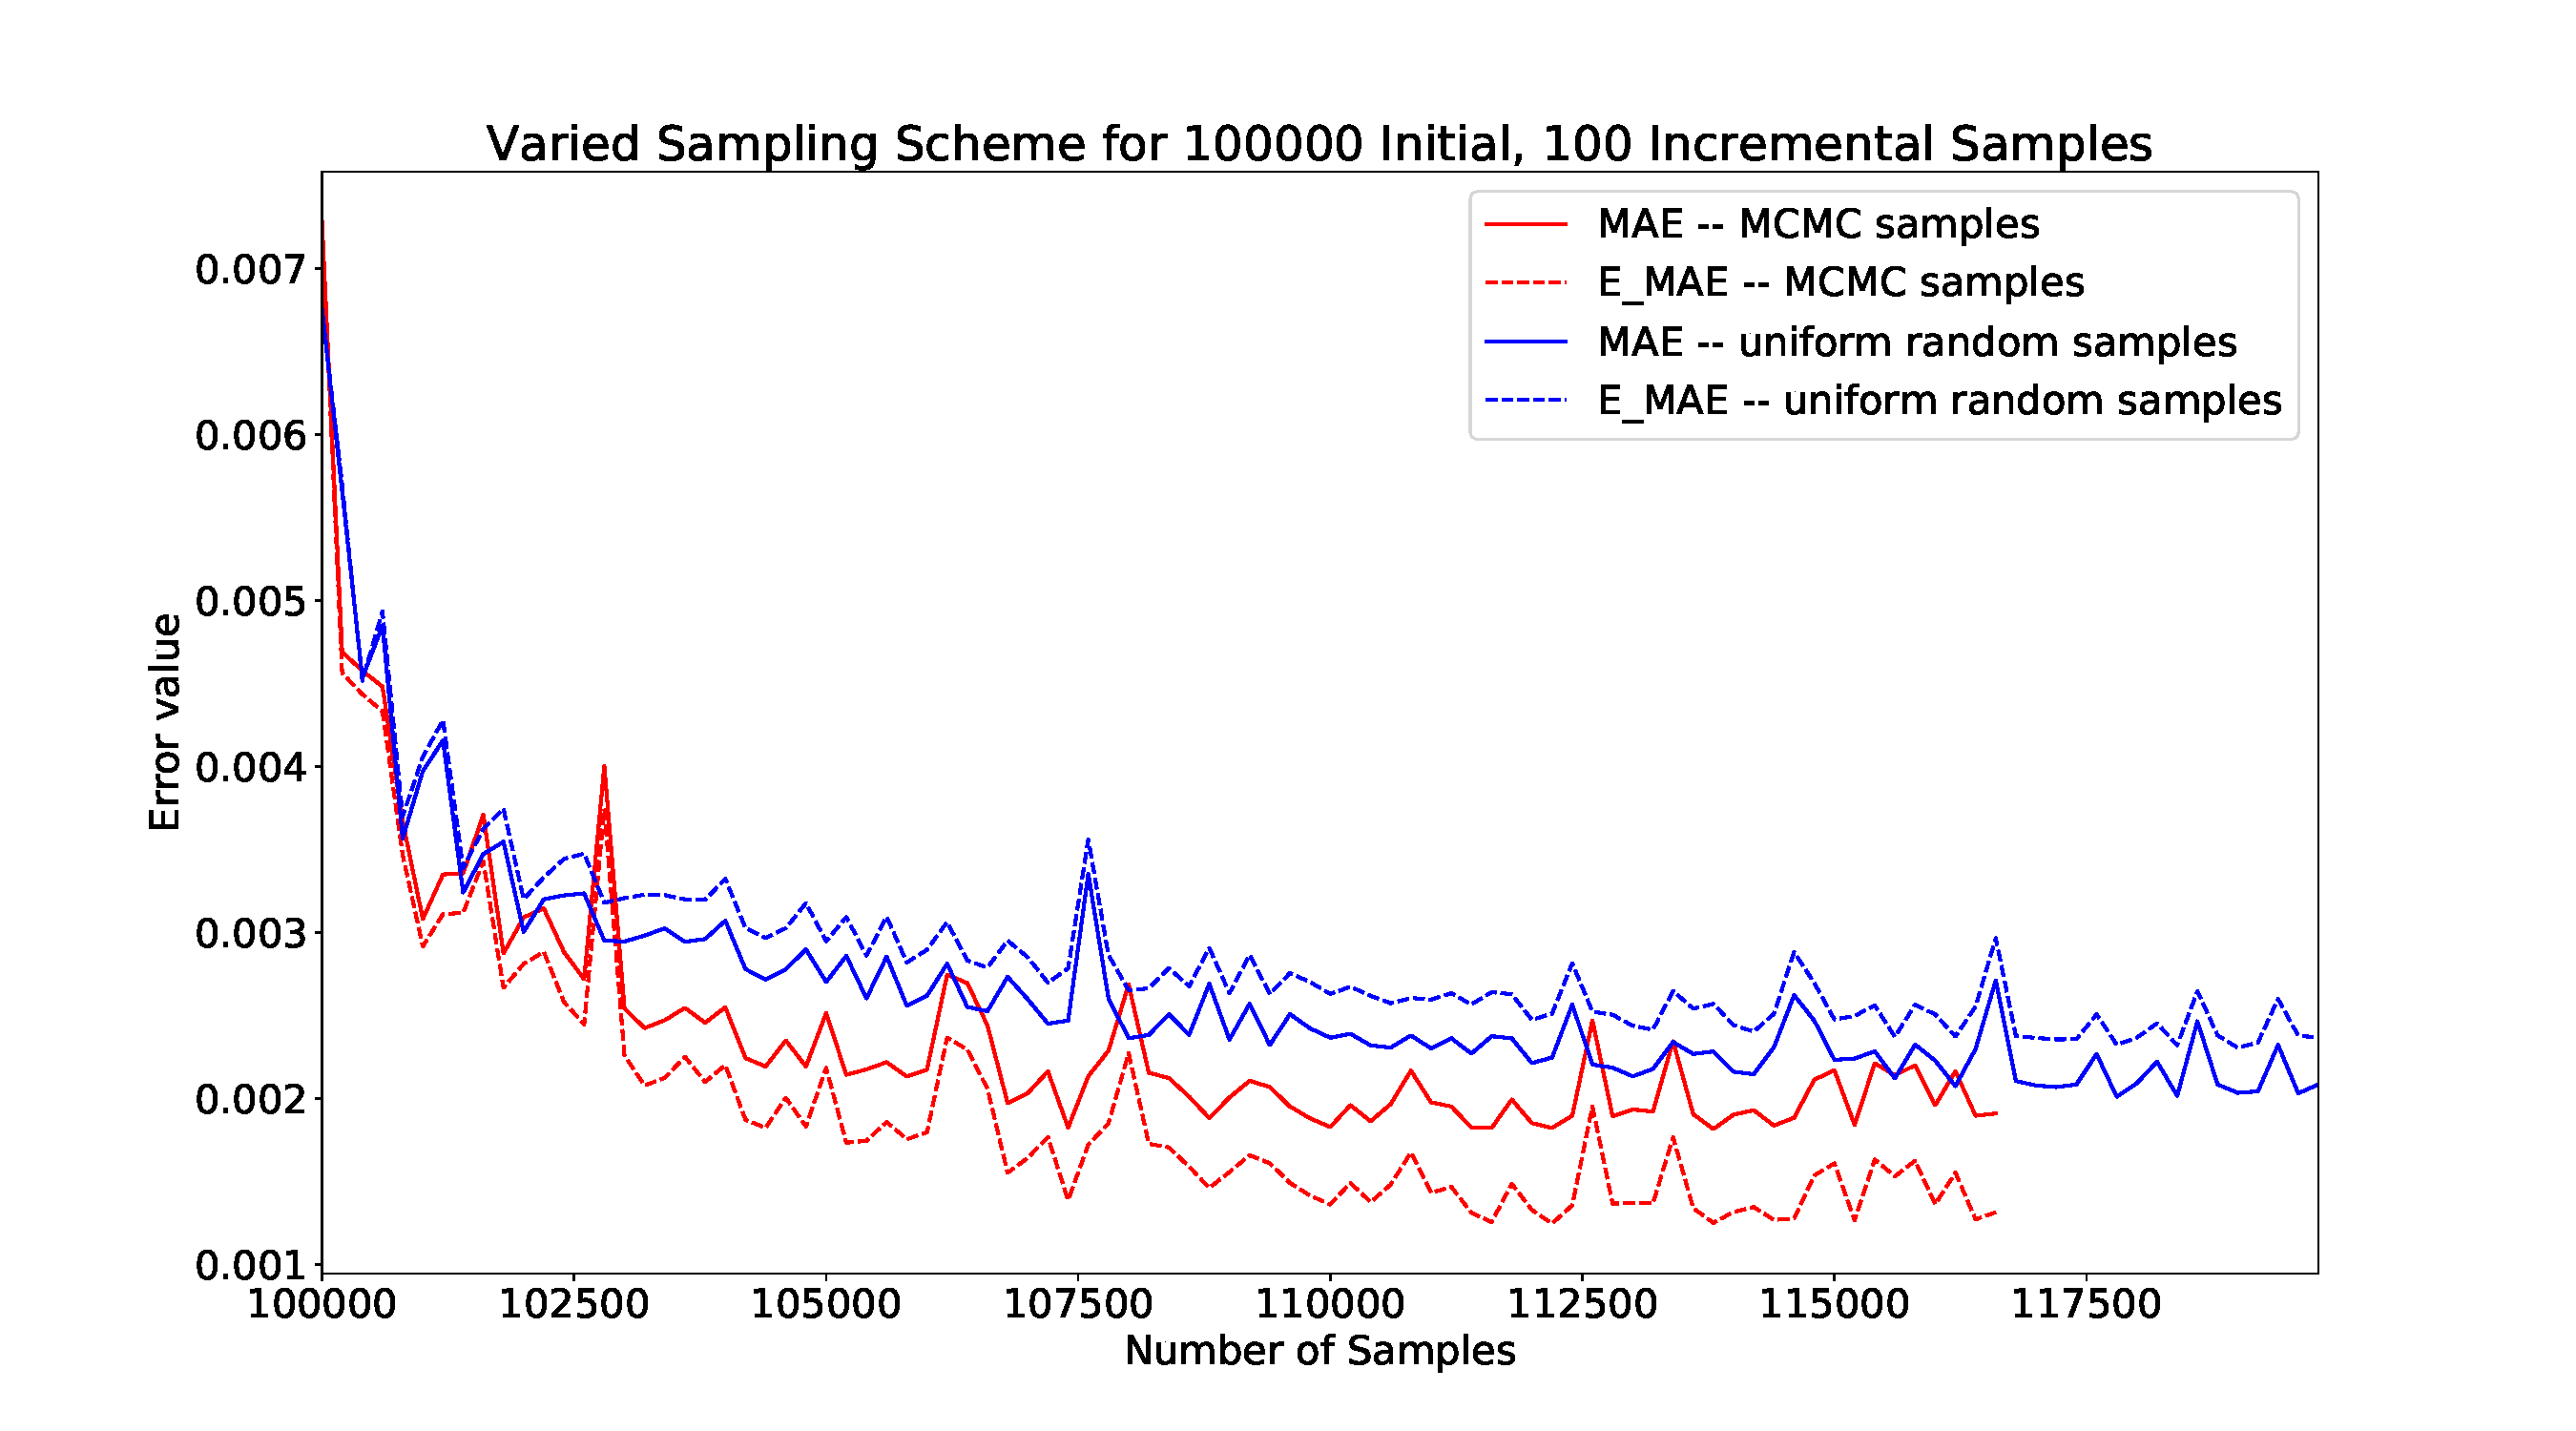
\includegraphics[width=12cm]{qassresult}
    \end{center}
    
    $60\%$ decrease in MAE for independent evaluation (dashed) \newline
    Equivalently, $6\%$ decrease in samples needed for same accuracy

\end{frame}

\begin{frame}
    \frametitle{Adaptive Sampling: Results}
    \vspace{-10pt}
    \begin{center}
    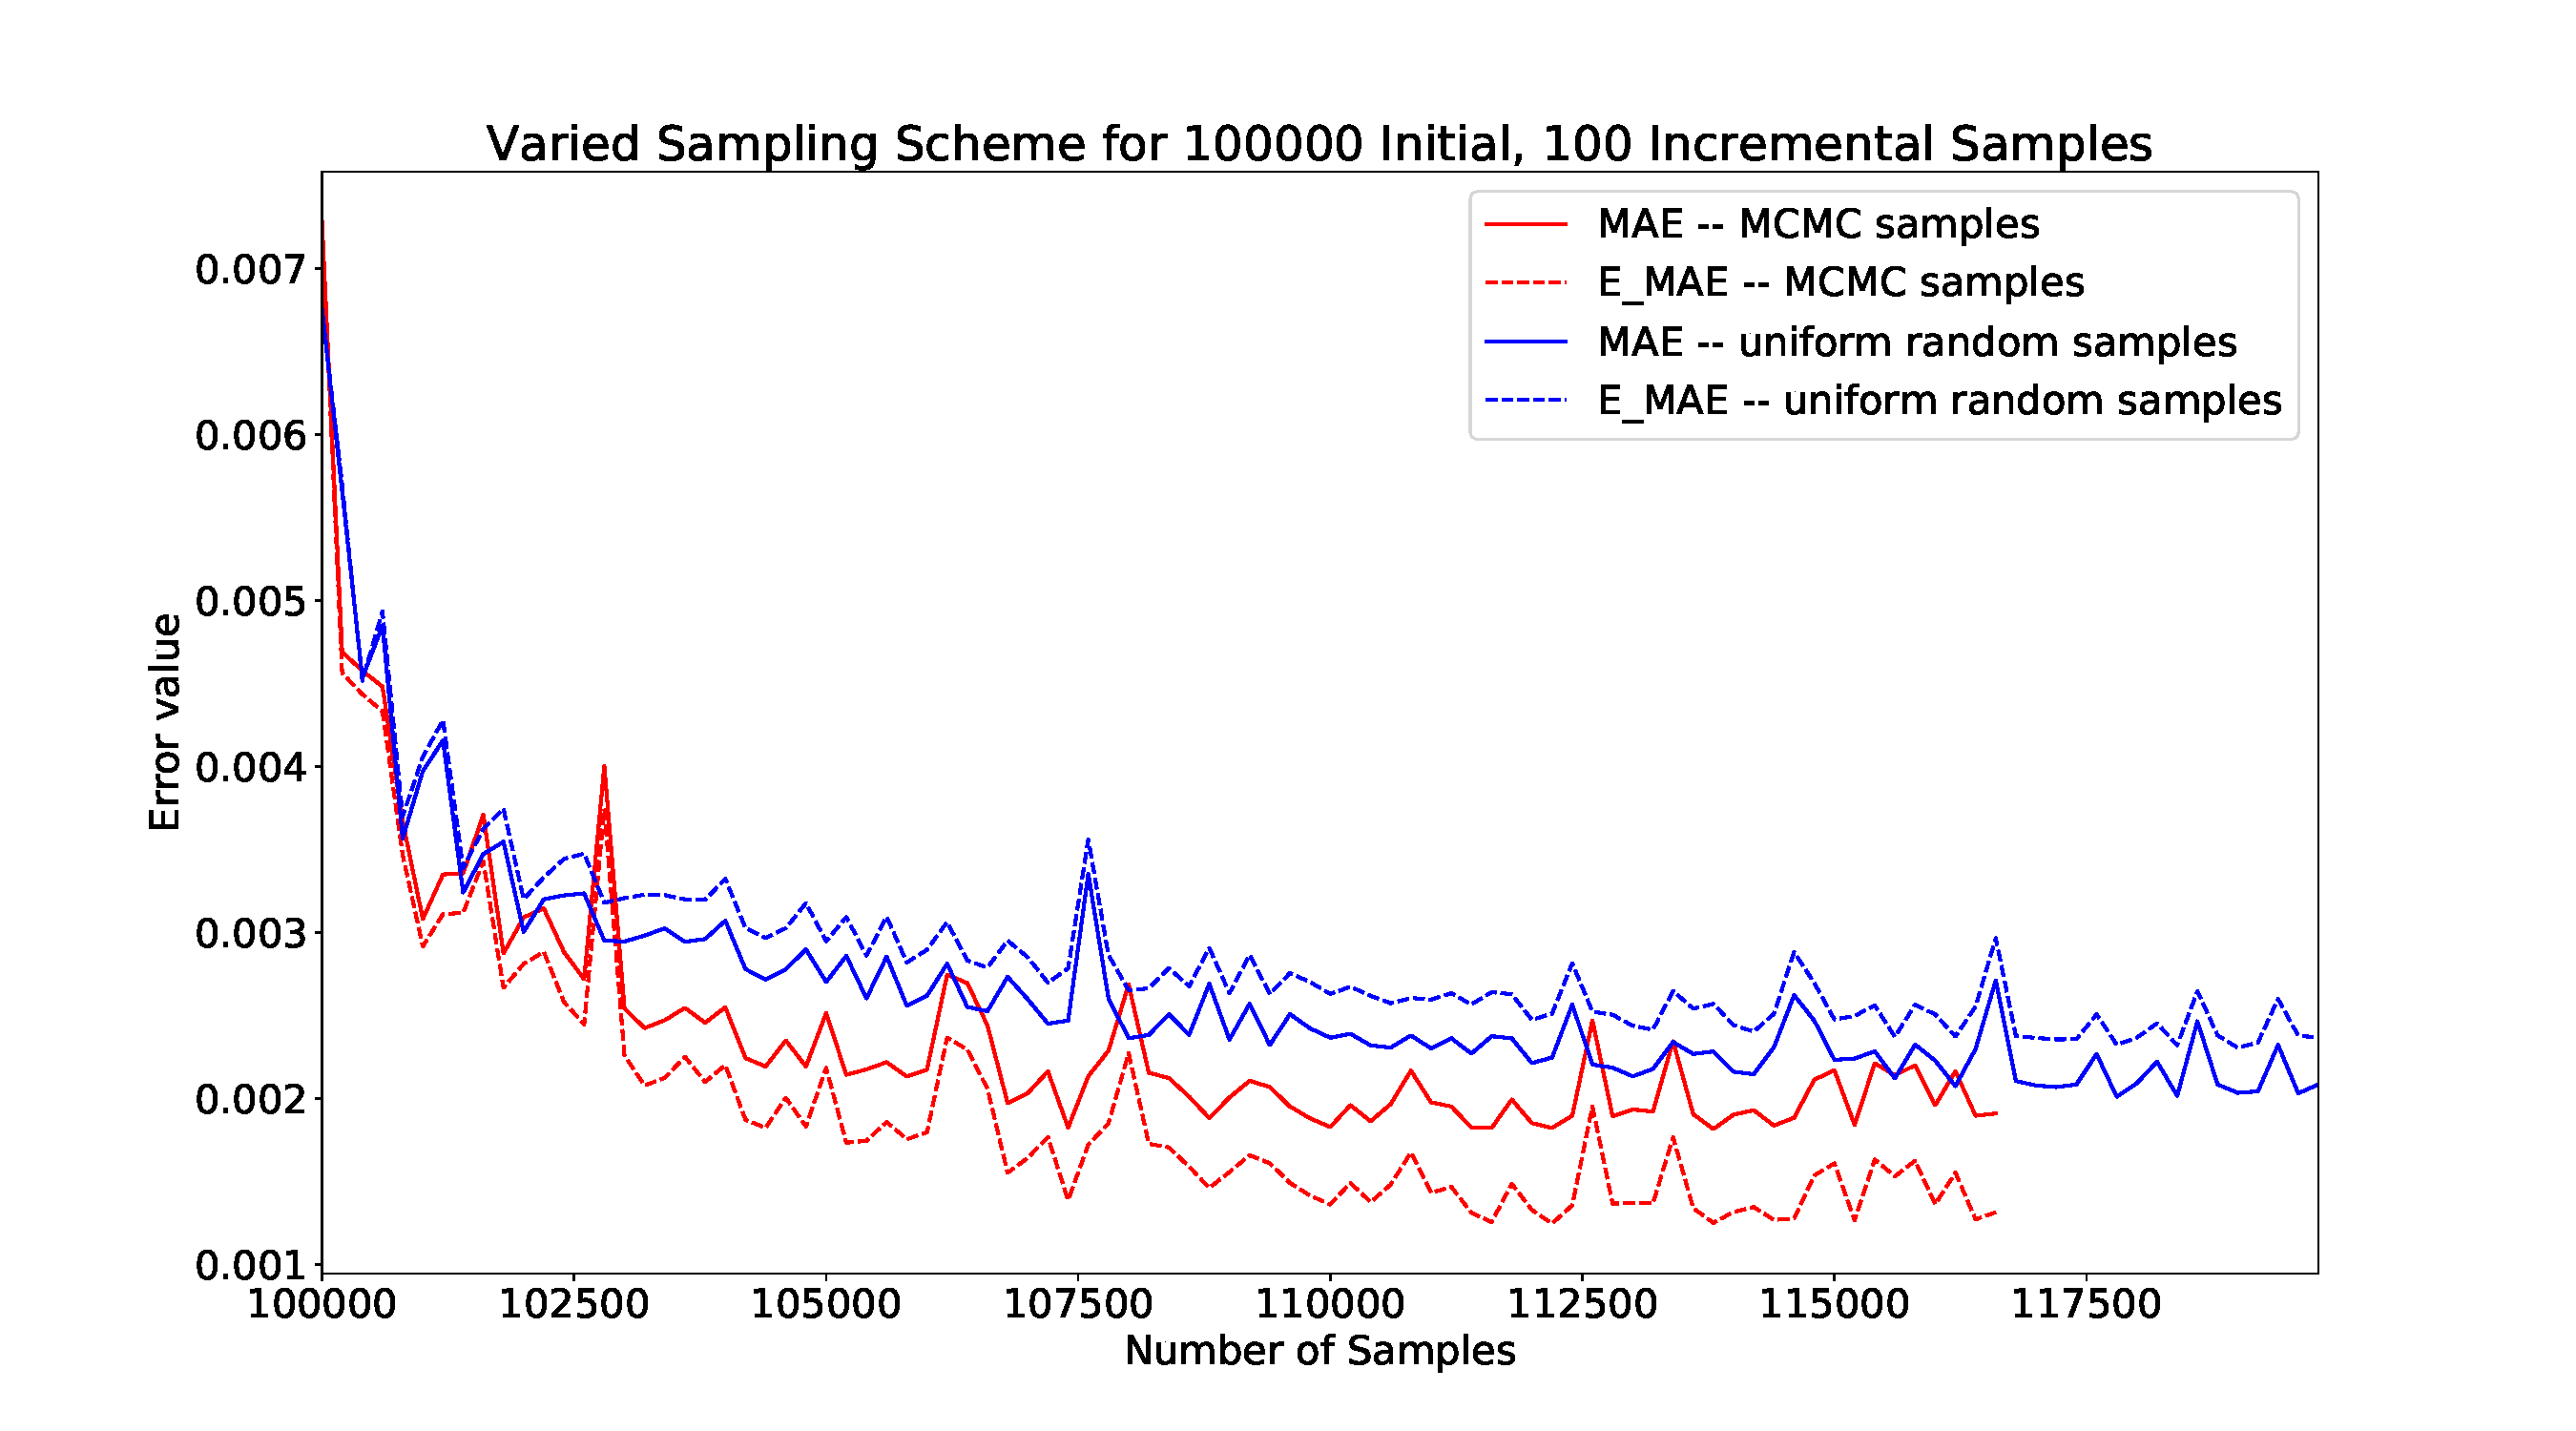
\includegraphics[width=12cm]{qassresult}
    \end{center}
    
    $60\%$ decrease in MAE for independent evaluation (dashed lines) \newline
    Equivalently, $6\%$ decrease in samples needed for same accuracy

\end{frame}

\begin{frame}
    \frametitle{Adaptive Sampling: Results}
    \vspace{-10pt}
    \begin{center}
    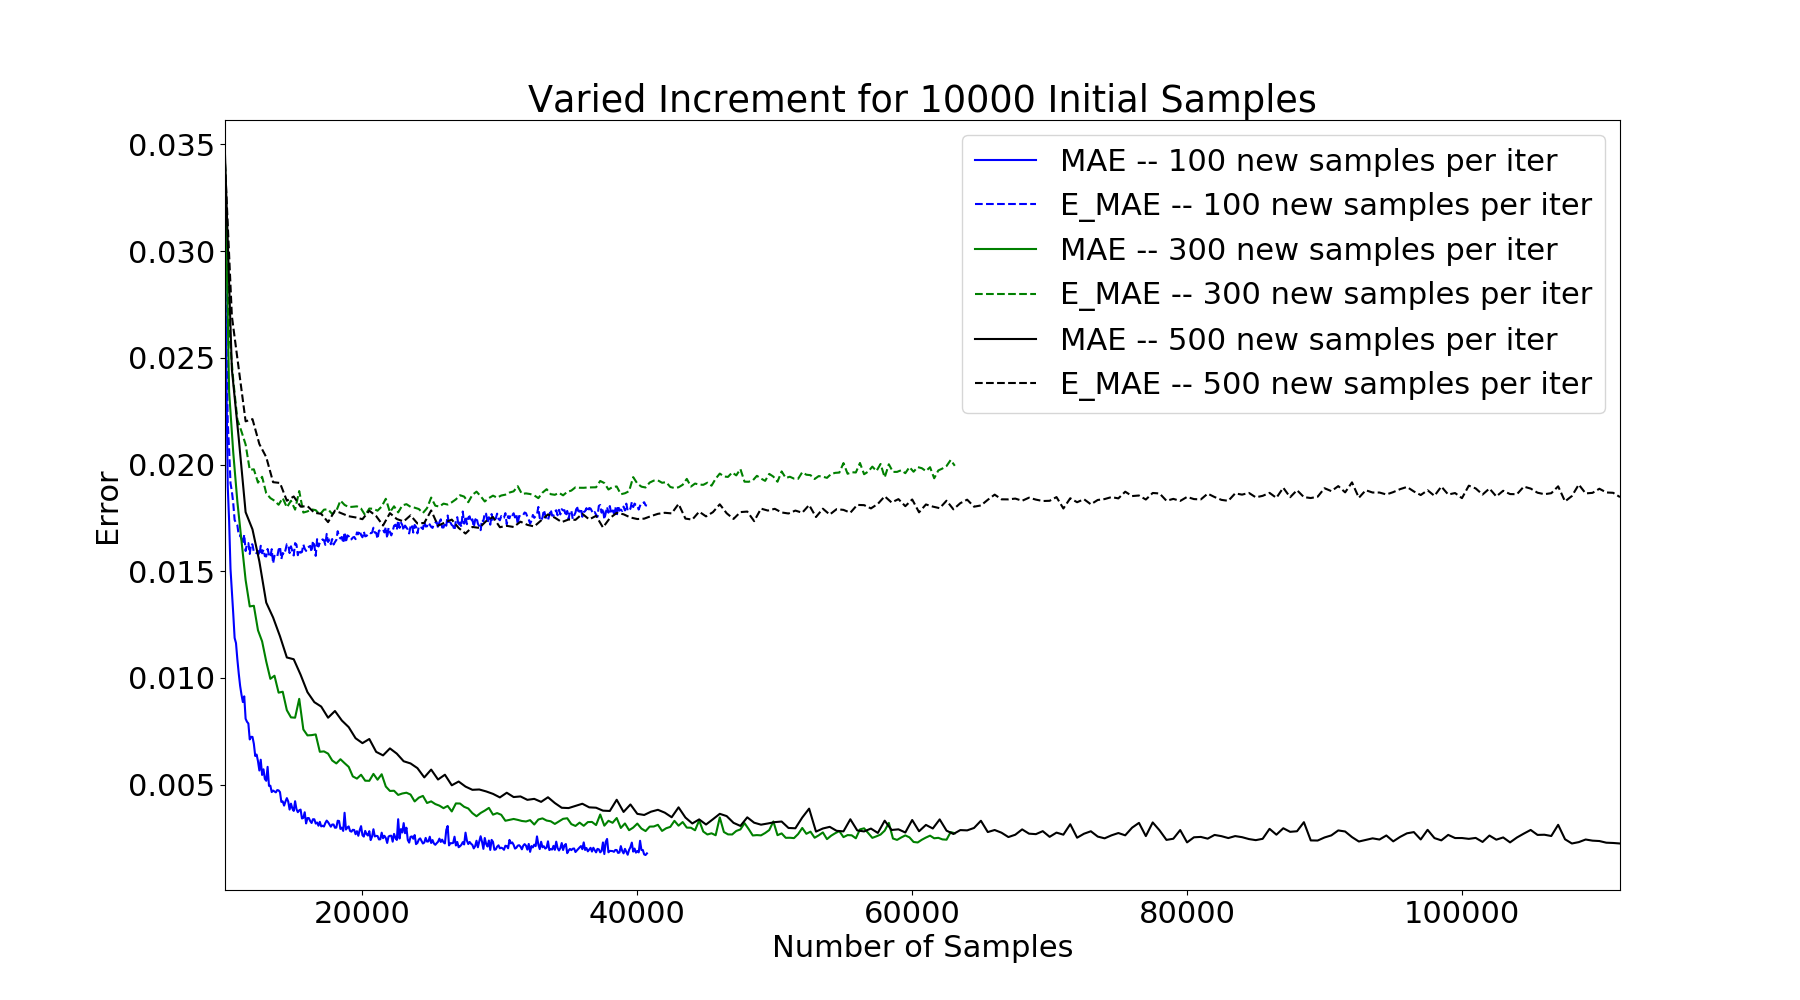
\includegraphics[width=12cm]{qassincr}
    \end{center}
    
    Fewer incremented samples can lead to better accuracy! \newline
    But depends on initial samples, specific model -- further study needed.

\end{frame}


\section{Conclusion}
\begin{frame}
	\frametitle{Conclusion}

	\begin{block}{Decoupled Approach}
		\begin{itemize}
			\setlength\itemsep{0em}
			\item
				Heuristic: \alert{GBTs} for $<10^4$~samples,
				\alert{ANNs} for $\geq10^5$~samples.
			\item
				Fastest found surrogate evaluates TBR in~\SI{0.898}{\micro\second}
				with error~$\num{0.033}$. This is roughly~\alert{$8\cdot
				10^6\times$~faster} than Paramak.
			\item
				Found surrogates with comparable properties with
				\alert{$\approx$10K~samples}.
		\end{itemize}
	\end{block}

	\begin{block}{Adaptive Approach}
		\begin{itemize}
			\setlength\itemsep{0em}
			\item
				New theoretical approach \alert{QASS} developed, based on MCMC.
			\item 
				\alert{$60\%$ decrease} in evaluation MAE demonstrated.
			\item
				\alert{$6\%$ decrease} in expensive TBR samples needed.
		\end{itemize}
	\end{block}

	\begin{itemize}
		\item 
			All methods \alert{portable} $\rightarrow$ cheap approximation of any simulation.
		\item
			Article in IOP \alert{Journal of Nuclear Fusion} (pending).
		\item
			Included as a benchmark in the \alert{SciML Collaboration}.
	\end{itemize}

\end{frame}



\end{document}
